\section{Advective-Reactive \texorpdfstring{$r$}{r}-process}\label{sec:ar_rprocess}

\jicom{This section is very much a work in progress. I kind of forget what we did. :p}

Advective-reactive nucleosynthesis is the generalization of the convective-reactive framework to include transport of material beyond convection.
In this work, we take the \texttt{SkyNet} post-processed trajectories \jitxt{done by Rodrigo ? citation ?} that escape a black hole formed by neutron star mergers and determine whether the advective-reactive framework is relevant to $r$-process nucleosynthesis.

Over time, the distance between any two trajectories increases as they move away from the black hole.
That means there is a time limit on how long the trajectories are able to exchange material.
We defin a distance $L_{\mathrm{mix}}$ analogously to $\ell_{\mathrm{mix}}$ and say that any two trajectories that are within this distance can exchange material.
\begin{equation}
    L_{\mathrm{mix}} = \sqrt{D t_{\mathrm{nuc}}}
\end{equation}
where $D=3\times10^16\mathrm{cm}^2/\mathrm{s}$ is the diffusion coefficient and $t_{\mathrm{nuc}}$ was given an analytic form based on an eyeballed linear fitting of  $\tau=X/(dX/dt)$ vs $t$ plots for some neutron heavy In isotopes.
Because of this, we get $L_{\mathrm{mix}}$ as a function time.
If for a time $t \geq t_{\mathrm{mix}}$ the pairwise distance between two trajectories is less than $L_{\mathrm{mix}}(t)$ then we say that they can exchange material. The results of this analysis are shown in Figure \ref{fig:frac_exchanging}.
It appears that 7.5-15\% of trajectories could be able to exchange material for the optimistic cases.

Much more work is needed to determine whether this matters because if both trajectories are in NSE they would have roughly the same pattern anyways.
We were in the early stages of seeing if we could post-process the trajectories with \texttt{ppn} rather than \texttt{SkyNet} and see if maybe we could figure out if the trajectories are exchanging and at least one is not in NSE.
Also we wanted to ask if the trajectories that were eaten by the black hole could've exchanged material with the ones that escaped.

\begin{figure}[htbp]
    \centering
    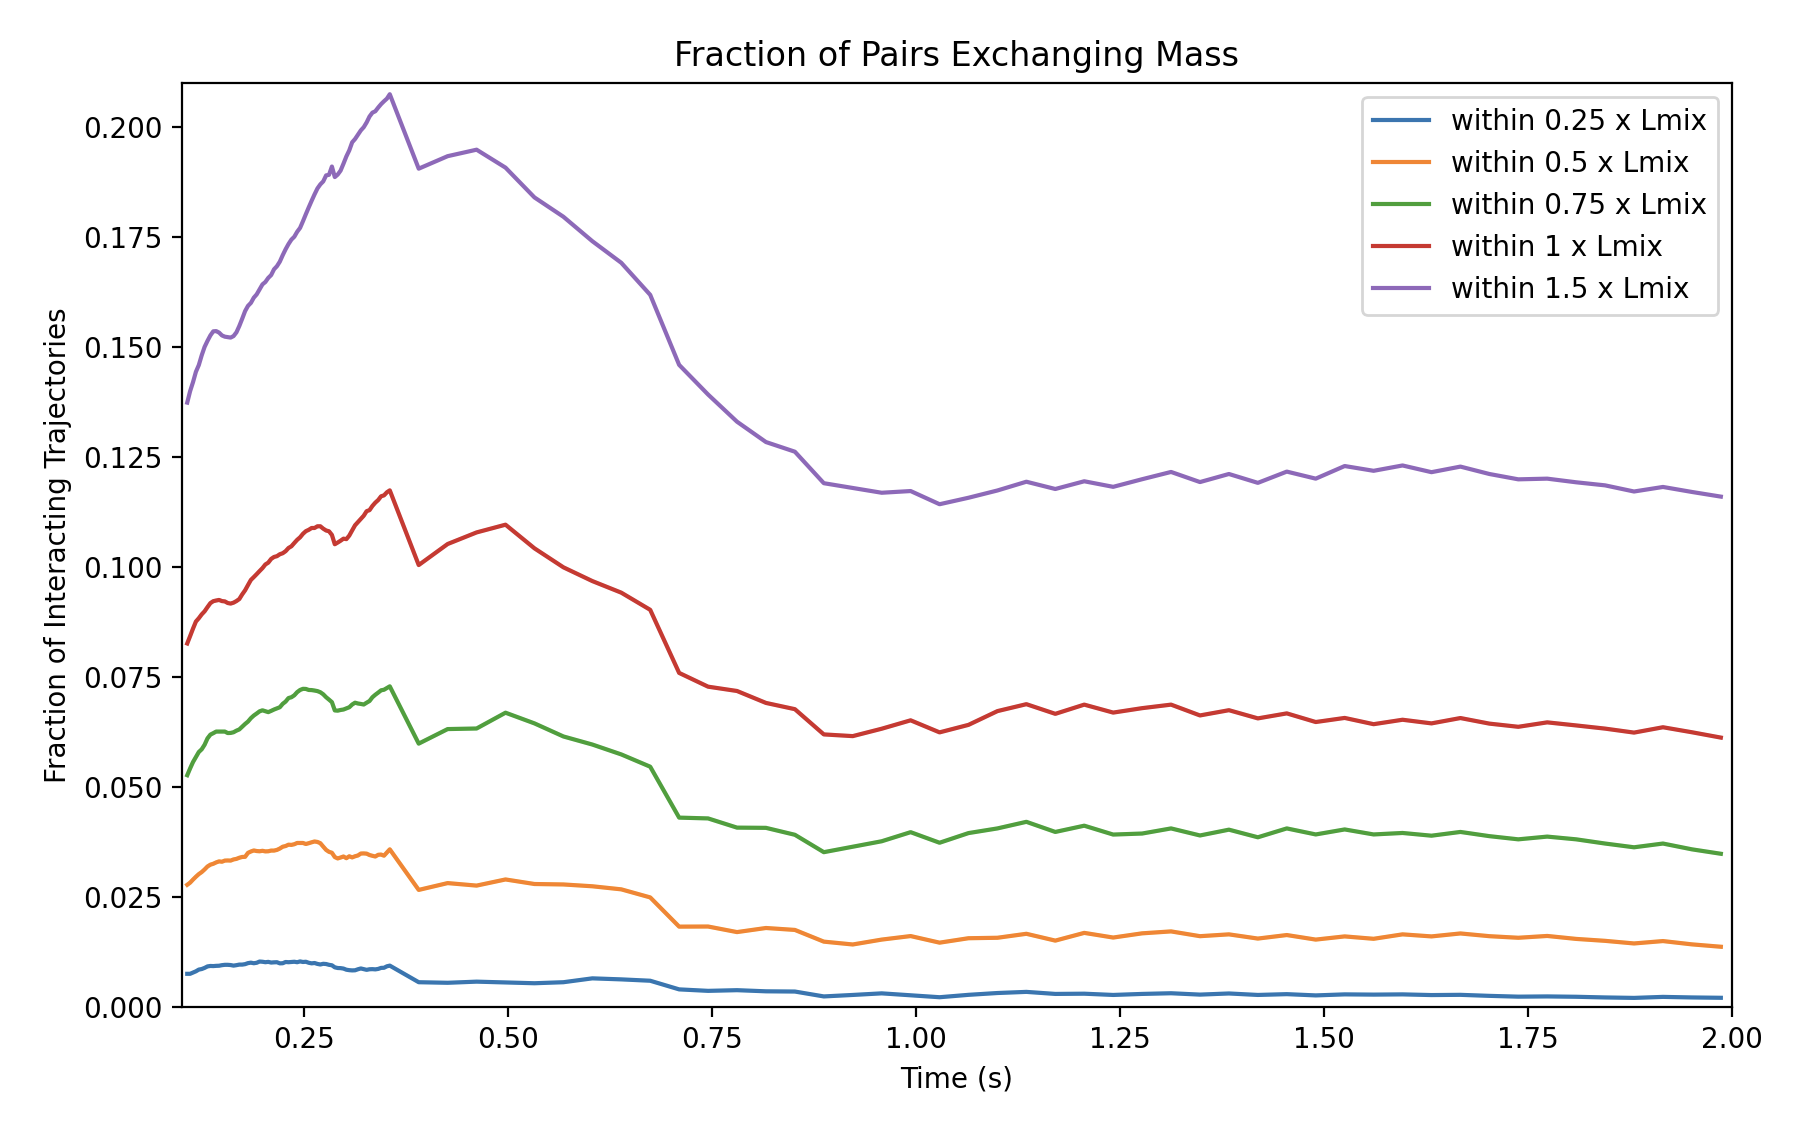
\includegraphics[width=\textwidth]{chapters/3/figures/frac_exchanging.png}
    \caption{Fraction of trajectories with distance for enough time to exchange mass. Each coloured line represents a size for $L_{\mathrm{mix}}$.
    \label{fig:frac_exchanging}}
\end{figure}